\documentclass[a4paper]{article}
\usepackage{graphics}
\usepackage[dvipdfmx]{graphicx}
\usepackage{bmpsize}
\usepackage{shonan}
\usepackage{hyperref}
\usepackage{tabularx}

\newcommand{\smallsection}[1]{\noindent \textbf{#1}. }

\begin{document}

% Generate a standard cover of an NII Shonan Meeting Report.
\SHONANno{152}
\SHONANtitle{Release Engineering for Mobile Applications}
\SHONANauthor{%
Shane McIntosh\\
Yasutaka Kamei\\
Meiyappan Nagappan}
\SHONANdate{December 09--12, 2019}
\SHONANmakecover

\title{Release Engineering for Mobile Applications}
\author{Organizers:\\
Shane McIntosh (McGill University, Canada)\\
Yasutaka Kamei (Kyushu University, Japan)\\
Meiyappan Nagappan (University of Waterloo, Canada)}
\date{December 9--12, 2019}
\maketitle

\section{Overview of the Meeting}

\subsection{Background}

Release engineering is the process that ships code changes from a developer's workspace to the end user.
It encompasses tools and technologies to accomplish continuous integration, deployment, delivery, and experimentation, such as build specifications, infrastructure-as-code, containerization, and many more.

In recent years, there has been a renewed interest in this area, driven by the need to deliver new content to users in a continuous fashion.
For example, popular web browsers like Mozilla Firefox and Google Chrome have shifted from slow, semi-annual releases to rapid, six-week release cycles.
In the domain of web applications, where control over the main delivery process is retained, industry has produced innovative techniques to achieve continuous delivery of new content.
These techniques allow for new content to be tentatively released (e.g., canary deployment), seamlessly released (or rolled back) without customer-facing downtime (e.g., blue-green deployment), and analytically evaluated with data from the field (e.g., A/B testing).

At the same time, mobile applications have become a typical means of delivering content to users. For example, recent market studies show that about four billion mobile devices are connected in 2017\footnote{\url{https://is.gd/OVPgze}} and predict that the global mobile app economy is expected to be worth \$157 billion by 2022.\footnote{\url{https://is.gd/61uIoy}}

\subsection{Challenges and Opportunities}

Rather than delivering content directly through the web browser, mobile app users install applications on their mobile devices (e.g., smartphones, tablets).
Release engineers need to deliver new releases from a software organization to app stores that curate mobile apps and make them available to users.
The existence of third-party app stores in the release path from software organization to user poses several challenges:

\begin{itemize}
\item Users must opt-in to an update of the client-side app in order for new content to be delivered. Releasing too quickly creates an overhead for users, since downloading and installing updates may slow down access to apps. Moreover, with the explosive growth of mobile app sizes, users may need to pay expensive data fees for large downloads on cellular networks.
\item App stores act as a bottleneck between software organizations and users, which may impose delays in the release process. For example, to prevent malware and exploit- vulnerable apps from impacting users, all of the apps that appear in the Apple app store need to be certified by an Apple technician. This certification process is slow, cumbersome, and expensive.
\end{itemize}

\subsection{Goals of the Meeting}

The purpose of this Shonan meeting is to bring together leading researchers and practitioners from the release engineering and mobile apps fields. The aim is not only to foster an exchange of ideas, but also to outline a clear set of concrete grand challenges and propose a roadmap for how those challenges can be met by future work.

A tangible outcome that we are aiming to produce is a manuscript that describes the grand challenges and our roadmap for future research.
For example, a foreseeable grand challenge is how software organizations can achieve crowd-based deployment strategies that have become so popular for web applications (e.g., canary and blue-green deployment) in a mobile setting.
The produced manuscript will be submitted as a vision paper to a conference or journal.

\clearpage

\section{Meeting Schedule}

\begin{bfseries}
Check-in Day: December 08 (Sun)
\end{bfseries}
\begin{itemize}
\item Welcome Banquet
\end{itemize}
\begin{bfseries}
{Day1: December 09 (Mon)}
\end{bfseries}
\begin{itemize}
\item Plenary: Introduction to the meeting
\item Plenary: Introductory lightning talks
\item Breakout: Breakout session 1 (Artefacts, Fragmentation, Human Aspects, Log Analysis)
\item Plenary: Reports and discussion on breakout session 1
\end{itemize}
\begin{bfseries}
Day2: December 10 (Tue)
\end{bfseries}
\begin{itemize}
\item Plenary: Planning for breakout session 2 
\item Breakout: Breakout session 2 (Definitions)
\item Plenary: Reports and discussion on breakout session 2
\item Plenary: Planning for breakout session 3
\item Breakout: Session 2 (Continuous Experimentation, Quality Assurance, Tools)
\item Plenary: Reports and discussion on breakout group 3
\item Demo: Julian Hardy
\end{itemize}
\begin{bfseries}
Day3: December 11 (Wed)
\end{bfseries}
\begin{itemize}
\item Plenary: Plan for breakout session 4
\item Breakout: Session 4 (Seeding Collaborative Projects)
\item Group photo shooting
\item Excursion and Main Banquet
\end{itemize}
\begin{bfseries}
Day4: December 12 (Thu)
\end{bfseries}
\begin{itemize}
\item Plenary: Reports and discussion from breakout session 4
\item Breakout: Session 5 (Solidifying Collaboration Plans)
\item Plenary: Meeting retrospective \& closing
\end{itemize}

\clearpage

\section{Plenary Talks}

\subsection{Walkthrough of Modern Release Analyics Workbench for Android Apps}

Julian Harty, Commercetest Limited/Open University, UK

TODO

\clearpage

\section{Breakout Group Discussions}

\subsection{Session 1: Exploring Topics of Interest}

\subsubsection{Artefacts for Release Engineering of Mobile Apps}

\smallsection{Participants}
Cuiyun Gao, Yasutaka Kamei, Li Li, Shane McIntosh, Sebastian Proksch

\smallsection{Discussion Points}
The problems discussed are not specific to mobile app stores, rather than to generic centralized app stores (like Steam Game Platform, MS Windows Appstore, etc.). We think that, to draw the line between an App Store and a regular package manager is the ability of users to review and rate the individual store elements.

\smallsection{Data Sources}
\begin{itemize}
    \item User facing
        \begin{itemize}
            \item social media (reddit, blogs, twitter, FB, forums)
        \end{itemize}
    \item Developer facing
        \begin{itemize}
            \item App Stores
                \begin{itemize}
                    \item Apple, Google, Steam (commercial)
                    \item F-Droid (probably not representative), Linux Package Managers ... (open source)
                \end{itemize}
            \item app releases (app lineage)
            \item commit history
            \item StackOverflow Discussion
            \item Android Framework Evolution
        \end{itemize}
    \item In between
        \begin{itemize}
            \item Logs
            \item Crash Reports
        \end{itemize}
\end{itemize}

\smallsection{Pipeline} Table \ref{table:release} shows the artifacts in each phase of release pipeline. The bold phases are the ones that can benefit most from the use of social media. We can use posts as indicators of the release process or to mine new requirements. The other phases are a black box for commercial apps. It is hard to study these, because we lack access to reliable sources.

In general, several research challenges have to be solved, like how to automatically map social media posts and apps.

\begin{table}[h] \label{table:release}
    \centering
    \caption{Release Pileline and artifacts}
    \begin{tabular}{l|l}
        \hline
        RelEng Phase & Artifacts \\ \hline 
        \textbf{Requirements Engineering} & social media, user         reviews \\ 
        Integration & Open Source App Stores (e.g., F-Droid) \\
        Build + Test & Git, CI Providers \\
        Deployment & app lineage \\
        \textbf{Monitoring + Reaction} & logs, social media, user
        reviews  \\ \hline
    \end{tabular}
\end{table}

\subsubsection{Overcoming Fragmentation of Android Versions in Deployment of Mobile Apps}

\smallsection{Participants} Carmine Vassallo, Keheliya Gallaba, Raula Gaikovina Kula, Li Li, Daniel Dominguez

\smallsection{Definitions} Push-based deployment model (in case of a web app): Build $\rightarrow$ Deploy $\rightarrow$ Release

Pull-based deployment model (in case of mobile apps): A pull request is generated when the app is submitted to the App Store. The App store can refuse/accept it as well as the user.

\smallsection{Challenges} 

\begin{itemize}
    \item For developers
        \begin{itemize}
            \item Misaligment on Frontend \& Backend
            \item Tracebility of app reviews to an app version (and therefore to a changelog)
            \item Tracebility between user and developer artifacts
            \item Can not force users to update
            \item Support legacy software
        \end{itemize}
    \item For researchers
        \begin{itemize}
            \item Lack of data for studies. In particular backend information
        \end{itemize}
\end{itemize}

\smallsection{Research directions}
\begin{itemize}
    \item Feature toggle updates to emulate canary updates (How to get them right and proper)
    \item Factors that drive changes and updates to the users (What is a good release note that make people want to update faster?)
    \item Usage of network logs for aproximating the backend behaviour Compare the behaviour of the webapp to the frontend against the same backend
\end{itemize}


\subsubsection{Human Aspects of Release Engineering for Mobile Apps}

\smallsection{Participants}
Tom Zimmermann, Daniel German, Mike Godfrey, Fabio Palomba, Pick Thongtanunam, Kla Tantithamthavorn, Toshiki Hirao, Al-Subaihin, Masanari Kondo

\smallsection{Contents (Figure \ref{figHumanAspects})}
Release engineering is not about bug fixes, but it's about social contract / interactions between users and developers. We break users into 2 types, i.e., new users and existing users. Are we in the age of release economics? We try to release apps to get more money (\$\$\$), get more users, and chage users' behaviors. For example, we are about to release a new version with bug fixes and updates but don't forget to pay \$5. So, we hypothesize that users can change release engineering, and release engineering can change users' behaviors.

\begin{figure}[h] \label{figHumanAspects}
  \centering
  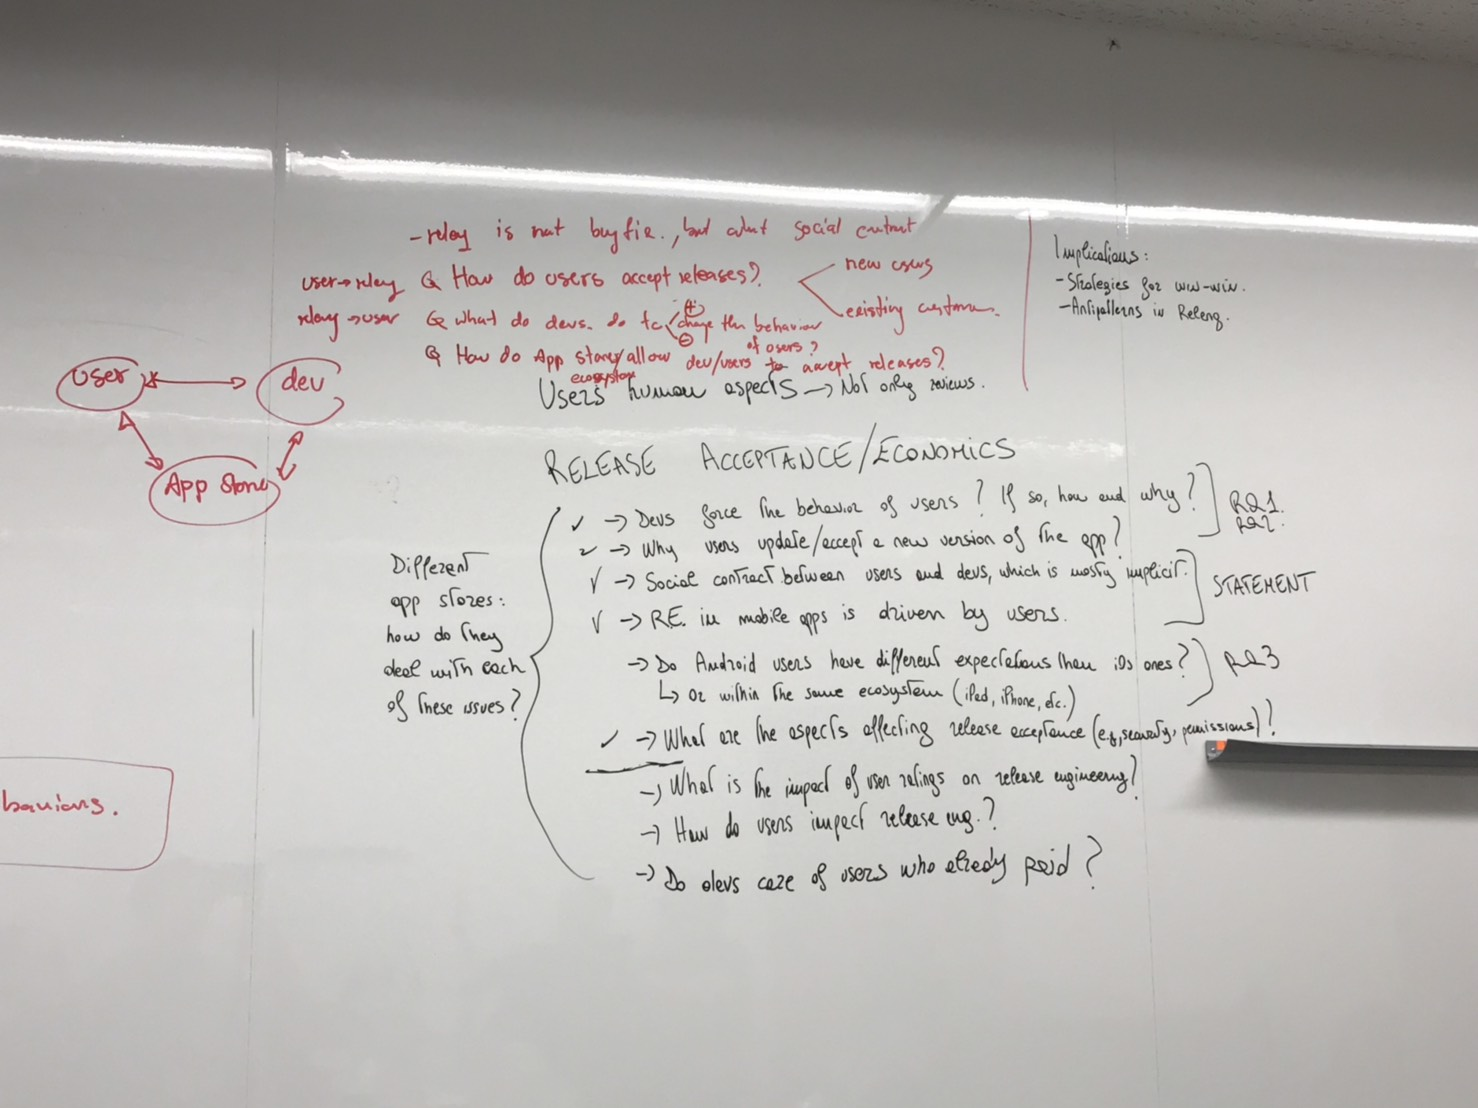
\includegraphics[width=0.7\columnwidth]{fig/day1.jpg}
  \caption{Brainstorming session for human aspects of release engineering for mobile apps}
\end{figure}

\begin{itemize}
    \item Q1: How do users accept releases (1st release for new users and later for existing users)? is it based on automatically updates?
    \item Q2: How do developers positively and negatively change the users' behaviors.
    \item Q3: How do app stores / ecosystems allow dev/users to accept releases?
    \item Implications/Benefits: win-win strategies for both users and developers + anti-patterns in release engienering.
    \item Other questions:
        \begin{itemize}
            \item Why mobile apps do not use issue tracking systems? Why do App stores do not provide ITSs for users?
            \item Do developers care about bugs?
            \item How do users accept releases?
            \item Do users care about security? What would users do or take to care about security? What are security-critical apps? (not all apps/users need to care about security)
            \item Do different app stores have different users' expectation / users' behaviors? (games have high reviews than educational app reviews)
            \item Why do the same apps but in different stores have different price?
            \item Do users from different app stores have different expectation/behaviors?
        \end{itemize}
\end{itemize}

\subsubsection{Log Analysis for Mobile Apps}



\subsection{Session 2: Establishing Working Definitions}

\subsubsection{Breakout Group A}

\subsubsection{Breakout Group B}

\subsubsection{Breakout Group C}

\subsubsection{Consensus}

\subsection{Session 3: The State of the Practice}

\subsubsection{Continuous Experimentation}

\subsubsection{Quality Assurance in the Realm of Release Engineering of Mobile Apps}

\subsection{Session 4 and 5: Seeding Collaborative Projects}

\subsubsection{Log Analysis}

\subsubsection{Continuous Experimentation with Mobile App Restrictions}

\subsubsection{The Ubiquity of the App Store Paradigm (Beyond Mobile Apps)}

\clearpage

\section{List of Attendees}

\subsection{Co-organizers}

\begin{itemize}
\item Shane McIntosh (McGill University, Canada)
\item Yasutaka Kamei (Kyushu University, Japan)
\item Meiyappan Nagappan (University of Waterloo, Canada)
\end{itemize}

\subsection{Meeting Participants}

\begin{itemize}
\item Afnan Al-Subaihin (King Saud University, Saudi Arabia)
\item Maur\'icio Aniche (Delft University of Technology, Netherlands)
\item Daniel Dominguez (IMDEA Software Institute, Spain)
\item Keheliya Gallaba (McGill University, Canada)
\item Cuiyun Gao (Nanyang Technology University, Singapore)
\item Daniel M. German (University of Victoria, Canada)
\item Mike Godfrey (University of Waterloo, Canada)
\item Julian Harty (Commercetest Limited/Open University, UK)
\item Toshiki Hirao (Nara Institute of Science and Technology, Japan)
\item Masanari Kondo (Kyoto Institute of Technology, Japan)
\item Raula Gaikovina Kula (NAIST, Japan)
\item Li Li (Monash University, Australia)
\item Fabio Palomba (University of Zurich, Switzerland)
\item Luca Pascarella (Delft University of Technology, Netherlands)
\item Sebastian Proksch (University of Zurich, Switzerland)
\item Weiyi Shang (Concordia University, Canada)
\item Chakkrit (Kla) Tantithamthavorn (Monash University, Australia)
\item Patanamon (Pick) Thongtanunam (University of Melbourne, Australia)
\item Carmine Vassallo (University of Zurich, Switzerland)
\item Lili Wei (The Hong Kong University of Science and Technology, China)
\item Thomas Zimmermann (Microsoft Research, USA)
\end{itemize}

\end{document}
